\chapter{Implementation of System}

\section{Initialization of the System}
The installation of the application is available on the google play store, the name of the application is InforMe@Dublin and is created under the company Smooth Solutions which is the name of which was created by the developer Adam O'Connor.

\section{Background to Android Devices Activity's Life-cycle} 

Regarding the activities on which each of these specific sections in the following chapter is based on a single activity page where all these methods are then utilised. The Android Activity Lifecycle is controlled by the use of seven individual methods of which are related to the android.app.Activity class which is a subclass of the ContextThemeWrapper class.

The activities in an Android app is just plainly a single screen in Android, or in another example just a window on a computer or a frame in creating Java applications. With the help of these activities, developers can then place all the UI components or widgets on this screen.

Below is a list of how each of the specific methods of an android application activity is used in figure - 7.1 as well as what each of the methods of the activity does which is located in the table - 7.1.

\begin{table}[!ht]
    \centering
    \caption{Activity Lifecycle}
    \label{Activity Lifecycle}
    \begin{tabular}{@{}llrl@{}}
        \toprule
        \multicolumn{1}{c}{\textit{Method}} & \textit{Description}\\ \midrule
        onCreate & called when the activity is first created \\ \midrule
         onStart & called when the activity is becoming visible to the user. \\ \midrule
         onResume & called when the activity will start interacting with the user. \\ \midrule
         onPause & called when the activity is not visible to the user. \\ \midrule
         onStop & called when the activity is no longer visible to the user. \\ \midrule
         onRestart & called after the activity is stopped, prior to start. \\ \midrule
         onDestroy & called when the activity is destroyed. \\ \bottomrule
    \end{tabular}
\end{table}

\begin{figure}[htbp]
    \center 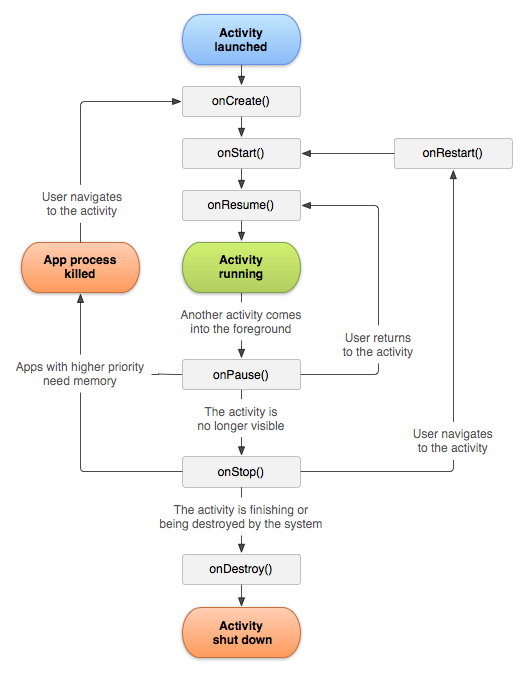
\includegraphics[width=350pt]{ActivityLife}\\
    \caption{Activity Life-cycle \cite{androidlife}} \label{Figure: Activity Life-cycle}
\end{figure}

\newpage

\section{Putting InforMe@Dublin Application on Google Play}
The informe app is signed with the author's credentials so that no intellectual information can be stolen or the application cannot be deconstructed by an unauthorised person to get the property of the developer. By uploading the application for reproduction on the Google play store the developer of informe had to gain the necessary SHA-1 encryption keys which were produced by the NSA used as a cryptographic hash function. The related encryption key creates a 160 bit or 20-byte hash value or also known as a message digest. 

\par The SHA-1 keys are needed to provide the related API keys on which are necessary for the usage of Google Maps as well as the OAuth used for the signing in of users authenticating with their Gmail account.
\newline
\textit{"C:\textbackslash Program Files (x86)\textbackslash Java\textbackslash jdk1.8.0\textunderscore 65 \textbackslash bin$>$ keytool -list -v -keystore "C:\textbackslash Users\textbackslash Adam O'Connor\textbackslash keyforInforMe\textbackslash InforMe@Dublin.jks" -alias     alias\textunderscore name -storepass password -keypass password"}

\begin{figure}[htbp]
    \center 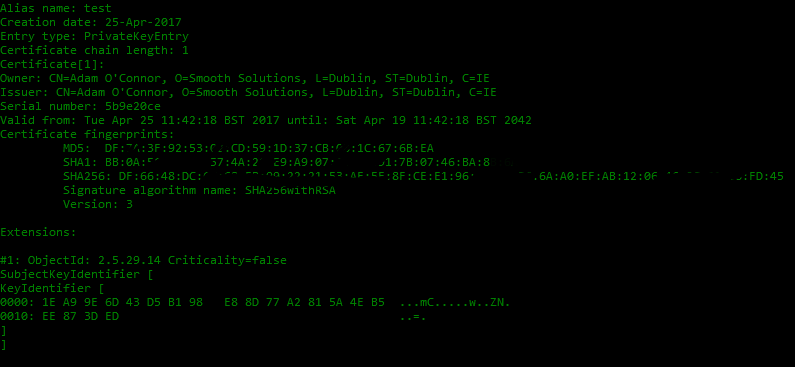
\includegraphics[width=450pt]{Hashkeys}\\
    \caption{Crypt Key Screenshot} \label{Figure: Crypt Key Screenshot}
\end{figure}

To obtain the SHA-1 key used in the generated signed APK the above console command is needed in order to retrieve the key which the developer needs to add to the Firebase database and OAuth 2 in both the Firebase console and Google API console. The Generated key store used to sign the application is needed to retrieve the SHA key. 

\section{A Way of allocating Permissions}
With regards to the new permissions that are now needed by applications to run on Android applications, a code listing was provided by the developer below. The new permissions were introduced by the Android development team with the release of Android marshmallow instead of users accepting terms of the downloaded application from the Google play store, and users would need to accept these permissions when needed throughout the use of such an application with are requested one by one. The developer has to call each request manually which is below.
\begin{lstlisting}[style=myCustomMatlabStyle, basicstyle=\small, breaklines, caption=Permissions Example,captionpos=b] 
 // check permission request of 99
 public static final int MY_PERMISSIONS_REQUEST_LOCATION = 99;
 
 /**
 * used to check the location permission
 * @return
 * dialog if user has not set permissions
 */
 public boolean checkLocationPermission() {
     if (ContextCompat.checkSelfPermission(this,
     Manifest.permission.ACCESS_FINE_LOCATION)
     != PackageManager.PERMISSION_GRANTED) {
     
         // Should we show an explanation?
         if (ActivityCompat.shouldShowRequestPermissionRationale(this,
         Manifest.permission.ACCESS_FINE_LOCATION)) {
         
             // Show an explanation to the user *asynchronously* -- don't block
             // this thread waiting for the user's response! After the user
             // sees the explanation, try again to request the permission.
             
             //Prompt the user once explanation has been shown
             //(just doing it here for now, note that with this code, no explanation is shown)
             ActivityCompat.requestPermissions(this,
             new String[]{Manifest.permission.ACCESS_FINE_LOCATION},
             MY_PERMISSIONS_REQUEST_LOCATION);
         
         
         } else {
             // No explanation needed, we can request the permission.
             ActivityCompat.requestPermissions(this,
             new String[]{Manifest.permission.ACCESS_FINE_LOCATION},
             MY_PERMISSIONS_REQUEST_LOCATION);
         }
             return false;
     } else {
         return true;
     }
 }
\end{lstlisting}
\par
The above code is used in conjunction with the requesting of the specific location permission of the device on which the app has been downloaded and opened. The location dialogue is the first permission on which would be shown to the user if the permission has not been set then the user cannot explicitly continue using the application. The dialogue module would simply keep showing until the user agrees to accept the location permissions. In conjunction with the checking location permissions method, an OnRequestPermissionsResult method is also used for the retrieval of such a permission request. The following method checks if the specific user has chosen to allow the app to receive the location of that app.
\newline
\begin{lstlisting}[style=myCustomMatlabStyle, basicstyle=\small, breaklines, caption=Permissions Request Example,captionpos=b] 
 /**
 *
 * @param requestCode
 * start to see if user connected
 * @param permissions
 * permissions which are needed for the application
 * @param grantResults
 * if the user has granted access to sensors.
 */
 @Override
 public void onRequestPermissionsResult(int requestCode,
 String permissions[], int[] grantResults) {
     switch (requestCode) {
         case MY_PERMISSIONS_REQUEST_LOCATION: {
             // If request is cancelled, the result arrays are empty.
             if (grantResults.length > 0
             && grantResults[0] == PackageManager.PERMISSION_GRANTED) {
             
                 // permission was granted, yay! Do the
                 // location-related task you need to do.
                 if (ContextCompat.checkSelfPermission(this,
                 Manifest.permission.ACCESS_FINE_LOCATION)
                 == PackageManager.PERMISSION_GRANTED) {
                 
                 }
         
            } else {
         
                 // permission denied, boo! Disable the
                 // functionality that depends on this permission.
                 checkLocationPermission();
             }
             return;
         }
         
         // other 'case' lines to check for other
         // permissions this app might request
     }
 }
\end{lstlisting}

\section{Utilising Firebase's Auth method}
Regarding the Firebase Auth method on which includes a user management system. With the following in mind, the developer can compare some basic data against the Firebase Auth users. Utilising the following method allows the developer to offer multiple login methods such as email/password, Google, Facebook. The following lets users link their accounts into a single Firebase account. Using the Auth method provides pre-existing auth system so that the application can take advantage of Firebase's security rules which have been set by the developer.

\section{Logging into Cloud services}
The cloud service on which this application connects to is Firebase. Firebase controls the authentication between the application itself and allows the signed in person to retrieve information which is located in the database. The following code was used in coordinance with the authentication with the following application.
\par
Email/password authentication has functions to register new users as well as signing them back in once registered. Firebase auth also provides a method of signing a user out of the application all functions return promises on which the new user registration as well as creating a profile on the database automatically signs the user in. The login information of the app is saved and holds the signing in information of the user if they have not signed out.

\begin{lstlisting}[style=myCustomMatlabStyle, basicstyle=\small, breaklines, caption=Authentication Example,captionpos=b] 

 /**
 * used for the signing in of a user which has logged in
 * with their email address and password.
 * @param email
 * email address of the user which created an account.
 * @param password
 * password on which user wants to use.
 */
 private void signIn(String email, String password) {
     Log.d(TAG, "signIn:" + email);
     // validate the textfields user has filled in.
     if (!validateForm()) {
        return;
     }
 
     showProgressDialog();
 
     // start the authentication of the email address and password of the user.
     final Task<AuthResult> authResultTask = mAuth.signInWithEmailAndPassword(email, password)
     .addOnCompleteListener(this, new OnCompleteListener<AuthResult>() {
         @Override
         public void onComplete(@NonNull Task<AuthResult> task) {
             Log.d(TAG, "signInWithEmail:onComplete:" + task.isSuccessful());
         
             if(task.isSuccessful()) {
                checkUserExistsDatabaseOnReEnter();
             }
             
             // If the sign in fails displays a message to the user. If sign in succeeds
             // the auth state listener will be notified and logic to handle the
             // signed in user can be handled in the listener.
             if (!task.isSuccessful()) {
                 Log.w(TAG, "signInWithEmail:failed", task.getException());
                 Toast.makeText(EmailPasswordAuthentication.this, R.string.auth_failed,
                 Toast.LENGTH_SHORT).show();
                 mStatusTextView.setText(R.string.auth_failed);
             }
         
            hideProgressDialog();
         }
     });
 }
\end{lstlisting}

The above method concludes the sign in of the application using the user's email and password to gain access to the following application. While choosing the sign in button after the user has entered their credentials the email and password will be used together with the use of Firebase Auth. The information is then sent to the Firebase project which is linked to the project utilising a google-services.json file of which is compromised of the client information of the app as well as the OAuth information which relates to the application. The google-services.json file will be added into the appendix in this chapter.
\par
With the following in mind, the  Google authentication of the users is used in the same way with some other methods used to map the OAuth 2 authentication together with the Google services API on which is automatically created in the Google console.  OAuth with web authentication is needed as it is a requirement of Android if the app is released on the Google play store as some instances are authenticated with the web authentication.
\newline

\begin{lstlisting}[style=myCustomMatlabStyle, basicstyle=\small, breaklines, caption=Google Authentication Example,captionpos=b] 
 // Configure Google Sign In
 GoogleSignInOptions gso = new GoogleSignInOptions.Builder(GoogleSignInOptions.DEFAULT_SIGN_IN)
     .requestIdToken(getString(R.string.default_web_client_id))//requesting the specific token the Google sign.
     .requestEmail() // requesting the email address of the user to sign in.
     .build();
 
 // creation of a Google API client for the connection of a Google token of the OAuth 2 API in the Google Console.
 mGoogleApiClient = new GoogleApiClient.Builder(this)
     .enableAutoManage(this, new GoogleApiClient.OnConnectionFailedListener() {
         @Override
         public void onConnectionFailed(@NonNull ConnectionResult connectionResult) {
         
         }
     })
     .addApi(Auth.GOOGLE_SIGN_IN_API, gso)// addtion of the Google sign in API and Google sign in options.
     .build();
 \end{lstlisting}

\section{Creation of User Preferences}
About the following section which utilises users preferences throughout the use of the InforMe@Dublin application. The developer will display some of the code of which is related to using user's preferences within an Android application environment the developer used preferences in informe by way of reusing the same activity but by producing different layouts to the user. Here is a following code listing of the preference method.

\begin{lstlisting}[style=myCustomMatlabStyle, basicstyle=\small, breaklines, caption=Preferences Example,captionpos=b] 

/**
* This fragment shows notification preferences only. It is used when the
* activity is showing a two-pane settings UI.
*/
@TargetApi(Build.VERSION_CODES.HONEYCOMB)
public static class NotificationPreferenceFragment extends PreferenceFragment {
    @Override
    public void onCreate(Bundle savedInstanceState) {
        super.onCreate(savedInstanceState);
        addPreferencesFromResource(R.xml.pref_notification);
        setHasOptionsMenu(true);
        
        // Bind the summaries of EditText/List/Dialog/Ringtone preferences
        // to their values. When their values change, their summaries are
        // updated to reflect the new value, per the Android Design
        // guidelines.
        
        bindPreferenceSummaryToValue(findPreference("notifications_new_message_ringtone"));
    }
}

\end{lstlisting}
With the code listing above on which was provided by the developer shows how the specific preferences are bound within the app.  As the user chooses to enter the settings activity, the following layout is provided upon request. Each of the two layout preference headers is used in conjunction with there specific layout files to produce to the user on request\newline
\begin{lstlisting}[style=myCustomMatlabStyle, basicstyle=\small, breaklines, caption=Preferences Header Layout Example,captionpos=b] 
<preference-headers xmlns:android="http://schemas.android.com/apk/res/android">

<!-- These settings headers are only used on tablets. -->

    // The following code snippet is used to produce the specific preference layout of Battery Saver
    <header
    android:fragment="adamoconnor.informe.Settings.SettingsActivity$DataSyncPreferenceFragment"
    android:icon="@drawable/batteryicon"
    android:title="Battery Saver" />

    // The following code snippet is used to produce the specific preference layout of Notification Preference.
    <header
    android:fragment="adamoconnor.informe.Settings.SettingsActivity$NotificationPreferenceFragment"
    android:icon="@drawable/ic_notifications_black_24dp"
    android:title="@string/pref_header_notifications" />

</preference-headers>
\end{lstlisting}
While the settings activity on which controls the following preference header's is extended to another class called AppCompatPreferenceActivity which itself extends PreferenceActivty is used to control and replace the view on which the user has chosen to use their personal preferences for the app. Users can choose the particular tone of the notification which will be sent to the user entering a Geofence. The other preferences the user of the app can choose to activate is the battery saver preference which will allow the screen of such a device to deactivate the screen display when the devices proximity sensor detects an object in front of it such as putting the device in the users pocket. This saves the battery life of the device which allows more time for exploring the InforMe@Dublin application.

\section{Retrieving of Google's Mapping System}
Within this following section of the implementation of the application is one of the most important tasks of the inforMe@Dublin application. Loading the map when the user chooses they want to display their location and to view the geofences in the area in which they are in. The map loading quickly and smoothly with regarding the users quality of play with the app is of utmost importance.Below is two code snippets of which are used to load the Google map onto the activity of the device asynchronously. The mapping resource is used as a fragment which is displayed over the event in question.
\begin{lstlisting}[style=myCustomMatlabStyle, basicstyle=\small, breaklines, caption=OnCreate Method Map Loading Example,captionpos=b] 

 mapFrag = (SupportMapFragment) getSupportFragmentManager().findFragmentById(map);
 mapFrag.getMapAsync(this);
 
\end{lstlisting}
Allowing for the integration of Google Maps into an Android application, a GoogleApiClient connection is needed on allowing the app to gain the necessary information to produce such a map fragment on the activity. The client of the ApiClient is initiated with the following code snippet below.
\begin{lstlisting}[style=myCustomMatlabStyle, basicstyle=\small, breaklines, caption=buildGoogleApiClient Code Snippet,captionpos=b] 

  /**
  * call the api client needed to retrieve information.
  * from google such as maps and the location API.
  */
  protected synchronized void buildGoogleApiClient() {
      mGoogleApiClient = new GoogleApiClient.Builder(this)
          .addConnectionCallbacks(this)
          .addOnConnectionFailedListener(this)
          .addApi(LocationServices.API)
          .build();
      mGoogleApiClient.connect();
  
  }

\end{lstlisting}
While loading the map fragment which is used in the InforMe@Dublin application to set specific UI components within the application, the developer can choose whether to show specific items within the map fragment. Within this section of the implementation, the developer has chosen to disable certain settings which then enables developer's to add their buttons or UI components which are then shown on the app. Within the section which enables certain UI components, the map type can be distinguished with layouts such as:
\begin{lstlisting}[style=myCustomMatlabStyle, basicstyle=\small, breaklines, caption=Map Types,captionpos=b] 

    mMap.setMapType(GoogleMap.MAP_TYPE_NORMAL);
    mMap.setMapType(GoogleMap.MAP_TYPE_SATELLITE);
    mMap.setMapType(GoogleMap.MAP_TYPE_TERRAIN); 
    mMap.setMapType(GoogleMap.MAP_TYPE_HYBRID);
\end{lstlisting}
Within the next code, listing below is how the map is asynchronously loaded within the application. The onMapReady method is called automatically when the actual map fragment is called upon.
\begin{lstlisting}[style=myCustomMatlabStyle, basicstyle=\small, breaklines, caption=Building the Map,captionpos=b] 

/**
* creating the map on the creation of the activity.
* set each of the UI components of the map, such as
* compass, etc.
* @param googleMap
* pass the map on which is being shown on the activity.
*/
@Override
public void onMapReady(GoogleMap googleMap) {

    mGoogleMap = googleMap;
    // type of map needed to display.
    mGoogleMap.setMapType(GoogleMap.MAP_TYPE_HYBRID);
    
    UiSettings uiSettings = googleMap.getUiSettings();
    uiSettings.setAllGesturesEnabled(true);
    uiSettings.setCompassEnabled(true);
    uiSettings.setMyLocationButtonEnabled(false);
    uiSettings.setMapToolbarEnabled(true);
    uiSettings.setZoomControlsEnabled(false);
    googleMap.setTrafficEnabled(false);
    
    //Initialize Google Play Services
    if (Build.VERSION.SDK_INT >= Build.VERSION_CODES.M) {
        if (ContextCompat.checkSelfPermission(this,
        Manifest.permission.ACCESS_FINE_LOCATION)
        == PackageManager.PERMISSION_GRANTED) {
            buildGoogleApiClient();
            mGoogleMap.setMyLocationEnabled(true);
        }
    } else {
        buildGoogleApiClient();
        mGoogleMap.setMyLocationEnabled(true);
    }
}

\end{lstlisting}

\section{Attaining Clients Correlative Location}
Regarding the location manager of which is needed to gain access to the location of the device is as follows on Acquiring the location manager of the device in question is not done by instantiating a LocationManager directly but by rather requesting an instance from the device by calling the following method getSystemService(Context.LOCATION\textunderscore SERVICE) which returns a new handler regarding a new LocationManager instance. While retrieving the user's location of the device permissions are needed to gain an accurate reading. With the following in mind, it is advised on using the GPS module together with an internet connection, With the application as follows an internet connection is needed by the user to use the app.
\begin{lstlisting}[style=myCustomMatlabStyle, basicstyle=\small, breaklines, caption=Location Request Settings,captionpos=b]

 /**
 * when requesting location, needs interval set and what accuracy
 * the developer wants to achieve.
 */
 protected void createLocationRequest() {
     
     mLocationRequest = new LocationRequest();
     mLocationRequest.setInterval(3000);
     mLocationRequest.setFastestInterval(5000);
     mLocationRequest.setPriority(LocationRequest.PRIORITY_HIGH_ACCURACY);
     
     LocationSettingsRequest.Builder builder = new LocationSettingsRequest.Builder()
     .addLocationRequest(mLocationRequest);
     
     mLocationSettingsRequest = builder.build();
 }
\end{lstlisting}

\par
The code snippet above provides a reference to the location gathering of the user's device on connecting to the following activity on which the method has placed the setting of the interval with regards to the updating of the current position every couple of seconds.
\begin{lstlisting}[style=myCustomMatlabStyle, basicstyle=\small, breaklines, caption=OnConnected Location updates,captionpos=b]

/**
* call to location updates on when the device changes
* coordinates, it is then updated on the map.
* @param bundle
* the information of the activity.
*/
@Override
public void onConnected(Bundle bundle) {
    
    if (ContextCompat.checkSelfPermission(this,
    Manifest.permission.ACCESS_FINE_LOCATION)
    == PackageManager.PERMISSION_GRANTED) {
        createLocationRequest();
        LocationServices.FusedLocationApi.requestLocationUpdates(mGoogleApiClient, mLocationRequest, this);
    }
}
\end{lstlisting}

\section{Finding the Corresponding Positions of Historic areas}
With regards to retrieving the geofences which are needed for the population of the UI components such as drawing a circle of the Geofence radius and the marker which is needed to see if the device has entered the Geofence in question. The snippet of code which is below shows the reference to the Firebase database which is then needed to retrieve a reference to the child nominator. The data on which is retrieved from the data snapshot is then split up and added into a HashMap.

\begin{lstlisting}[style=myCustomMatlabStyle, basicstyle=\small, breaklines, caption=Reteriving text Information of Monument,captionpos=b]

 /**
 * creation of new firebase reference which populates an array of the specific,
 * populates with the specific name of the area and the coordinates
 */
 DatabaseReference database = FirebaseDatabase.getInstance().getReference();
 final DatabaseReference myRef = database.child("geofences").child(town.toLowerCase());
 myRef.addListenerForSingleValueEvent(new ValueEventListener() {
     @Override
     public void onDataChange(DataSnapshot alerts) {
         
         for (DataSnapshot alert : alerts.getChildren()) {
             String myLandmarks = alert.getValue().toString();
             //splitted name | long | lat
             String[] splited = myLandmarks.split("\\|");
             // send to the package com.example.adamoconnor.test02maps.LoginAndRegister; Constants Landmarks Hashmap.
             LANDMARKS.put(splited[0], new LatLng(Double.parseDouble(splited[1]), Double.parseDouble(splited[2])));
         }
     }
     @Override
     public void onCancelled(DatabaseError databaseError) {
         
     }
 });
 \end{lstlisting}
 \par
 While the code above retrieves the Geofences and populates each of the historical places into a HashMap, the MapsActiviy is used in conjunction which displays each of these monuments coordinates on the map fragment. The snippet below is how these Geofences are populated. Keep in mind of which a reference of an ArrayList is then added which is populated with the information of the Landmarks Hashmap. The ArrayList in this instance is needed to see when the user's device in question is within the Geofence radius which in this case is 50 meters.
 
\begin{lstlisting}[style=myCustomMatlabStyle, basicstyle=\small, breaklines, caption=Displaying of Geofences,captionpos=b]
 
/*
* used for the loading of all geofences which where called from firebase when
* the user has signed in.
*/
for (Map.Entry<String, LatLng> entry : adamoconnor.informe.MapsAndGeofencing.Constants.LANDMARKS.entrySet()) {
      
      // creation of the geofence colour and border colour.
     // setting of each specific geofence.
      CircleOptions circleOptions = new CircleOptions()
           .center(new LatLng(entry.getValue().latitude,entry.getValue().longitude))
           .strokeColor(Color.argb(50, 70,70,70))
           .fillColor(getResources().getColor(R.color.Geofence))
           .radius(50);
      mGoogleMap.addCircle( circleOptions );
      
      //Place current location marker
      LatLng geo = new LatLng(entry.getValue().latitude,entry.getValue().longitude);
      MarkerOptions markerOptions = new MarkerOptions();
       markerOptions.position(geo);
       markerOptions.title(entry.getKey());
       markerOptions.icon(BitmapDescriptorFactory.fromResource(R.drawable.informe));//BitmapDescriptorFactory.defaultMarker(BitmapDescriptorFactory.HUE_MAGENTA)
      
      //adding marker to each geofence.
      mGeofenceMarker = mGoogleMap.addMarker(markerOptions);
      
      // add each to the geofence array list with the lat and long as well as the radius in meters.
      mGeofenceList.add(new Geofence.Builder()
           .setRequestId(entry.getKey())
           .setCircularRegion(
           entry.getValue().latitude,
           entry.getValue().longitude,
           adamoconnor.informe.MapsAndGeofencing.Constants.GEOFENCE_RADIUS_IN_METERS)
           .setExpirationDuration(adamoconnor.informe.MapsAndGeofencing.Constants.GEOFENCE_EXPIRATION_IN_MILLISECONDS)
           .setTransitionTypes(Geofence.GEOFENCE_TRANSITION_ENTER |
           Geofence.GEOFENCE_TRANSITION_EXIT)
           .build());
}
\end{lstlisting}
\par
Concerning the above code located in listing 6.14. The reader can then understand on how each geofence is loaded and then decoded into its specific geo-location. Each location is allocated a distinguishable marker from the Informe application with this in mind on selecting the marker of the area displays the name of the historical monument in question. The user can toggle to view these markers which open an option on getting directions of a monument of their choosing. Selecting this option will open up Google maps with the travel time etc. of the location.

\section{A Look at the Geofencing Notification Service}
When a user's device has received a location or the location has changed the developer has created a method to which calls the Geofencing request to see whether the user has entered that specific geofence on initiation. The following method is called in the code listing below.
\begin{lstlisting}[style=myCustomMatlabStyle, basicstyle=\small, breaklines, caption=Population of Geofences,captionpos=b]

/**
* used to see if user has entered a geofence.
*/
public void PopulateGeofences() {
    if (!mGoogleApiClient.isConnected()) {
        Toast.makeText(this, "Google API Client not connected!", Toast.LENGTH_SHORT).show();
        return;
    }
    
    try {
        LocationServices.GeofencingApi.addGeofences(
        mGoogleApiClient,
        getGeofencingRequest(),
        getGeofencePendingIntent()
        ).setResultCallback(this); // Result processed in onResult().
    } catch (SecurityException securityException) {
        // Catch exception generated if the app does not use ACCESS_FINE_LOCATION permission.
    }
}
\end{lstlisting}

While reading through the different implementations of some of the most important parts of the application the following section represents how notifications are initiated when a device enters such a location. While each of the HashMaps Geofences is loaded, they are also added to an ArrayList and sent to the GeofencingRequest method which allows for the checking if the device enters a geofence.

\begin{lstlisting}[style=myCustomMatlabStyle, basicstyle=\small, breaklines, caption=Geofence Request and Pending Intent,captionpos=b]

/**
* get the geofence which is requested.
* @return
* to the pending intent.
*/
private GeofencingRequest getGeofencingRequest() {
    GeofencingRequest.Builder builder = new GeofencingRequest.Builder();
    builder.setInitialTrigger(GeofencingRequest.INITIAL_TRIGGER_ENTER);
    builder.addGeofences(mGeofenceList);
    return builder.build();
}

/**
* sending the notification to the user when geofence is entered.
* @return
*/
private PendingIntent getGeofencePendingIntent() {
    
    Log.d(TAG, "Geo fence pending intent");
    Intent intent = new Intent(this, GeofenceTransitionsIntentService.class);
    // We use FLAG_UPDATE_CURRENT so that we get the same pending intent back when calling addgeoFences()
    
    return PendingIntent.getService(this, 0, intent, PendingIntent.FLAG_UPDATE_CURRENT);
}
\end{lstlisting}

\section{Retrieving Information of Historical Monuments}
With regards to the implementation of loading the historical monuments within the application was coded as follows by the developer of the following project. While the user of the device enters a geofence location with the intention of a notification looming on entering the geofence, that is produced with a pending intent. When a pending intent has then initiated a notification is then sent to the user's device of which is retrieved by the MapsActivity. If the user is using the app at the time or the user can simply choose to click the notification and be sent to the information activity which will show the subsequent history of that location. With that in mind, the name of the monument name is passed to a set variable which is located in the Place class.

\begin{lstlisting}[style=myCustomMatlabStyle, basicstyle=\small, breaklines, caption=Loading Information of Monuments,captionpos=b]

 /**
 * load the specific data of the historic information
 * this method retrieves the text for the activity
 * with a reference to load images.
 */
 private void LoadData() {
     
     //reference to Firebase database.
     DatabaseReference myRef = database.child("ruin");
     myRef.addValueEventListener(new ValueEventListener() {
         @Override
         public void onDataChange(DataSnapshot dataSnapshot) {
             
             //reference to load images method.
             informationImages();
             
             try {
                 
                 String info = (dataSnapshot.child(getMonumentName().trim()).getValue().toString());
                 title.setText(monumentName.trim());
                 String regex = "\\[|\\]";
                 info = info.replaceAll(regex, "");
                 information.setText(info);
                 
             } catch(NullPointerException ex) {
             LoadData();
         }
         
     }
     
     @Override
     public void onCancelled(DatabaseError databaseError) {}
     
 });
}
\end{lstlisting}
\par
With hence to the code located above the reader can see where the developer has provided a reference to the tree node of the Firebase database of which the following activity must have access to.  After the reference connection has been completed the monument name of the intent is passed to the informationFrontFragment on which populates the information text field with the appropriate text allocated in the Firebase database. When the following information has been retrieved the developer then has to perform a regex to remove certain elements from the text on which the Firebase database add's brackets to multiple lines of text.
\par
With regards to retrieving the images of which are related to a monument is compromised in a similar way to retrieving the child node of the parent in the database. For the population of each of the images, they are then compiled into a hash map and given a unique identity which is provided by a counter. These image URLs which are allocated by their monuments name and value of which were retrieved are then added onto a sliderLayout which will be changed every three seconds. The following code listing - 6.18 represents the loading of these images from the HashMap.

\begin{lstlisting}[style=myCustomMatlabStyle, basicstyle=\small, breaklines, caption=Loading Images on InformationFrontActivity,captionpos=b]

 Hash_file_maps = new HashMap<>();
 
 // load the images add numbers.
 int count = 1;
 for(DataSnapshot alert : alerts.getChildren()) {
     // pass the monument name
     Hash_file_maps.put(monumentName.trim()+", "+count, alert.getValue().toString());
     count++;
 }
 
 // add the images to the slider.
 for(String name : Hash_file_maps.keySet()) {
     
     TextSliderView textSliderView = new TextSliderView(getContext());
     
     textSliderView
         .description(name)
         .image(Hash_file_maps.get(name))
         .setScaleType(BaseSliderView.ScaleType.Fit)
         .setOnSliderClickListener(InformationFrontFragment.this);
         
     textSliderView.bundle(new Bundle());
     
     textSliderView.getBundle()
         .putString("extra",name);
     sliderLayout.addSlider(textSliderView);
     
 }
\end{lstlisting}

\section{Storage of Data}
With regards to the storing of the InforMe@Dublin information as well as each specific geofence location that is to be loaded onto a mapping application. Firebase is the answer to all of the questions while utilising the power of Firebase with regards to the security and anonymity of each specific user's data with reference to the users passwords and email address's all of these privacy issues are dealt with the Firebase console the developer doesnt have access to any password of which patrons of the application has set these are only reference by the unique identity key.

While the JSON data is added into the Firebase database the image below is what the InforMe@Dublin database actually look's like while the methods above show the retrieval of information from the database. Each line of these strings are associated with a corresponding parent.

\begin{figure}[htpb]
	\centering
	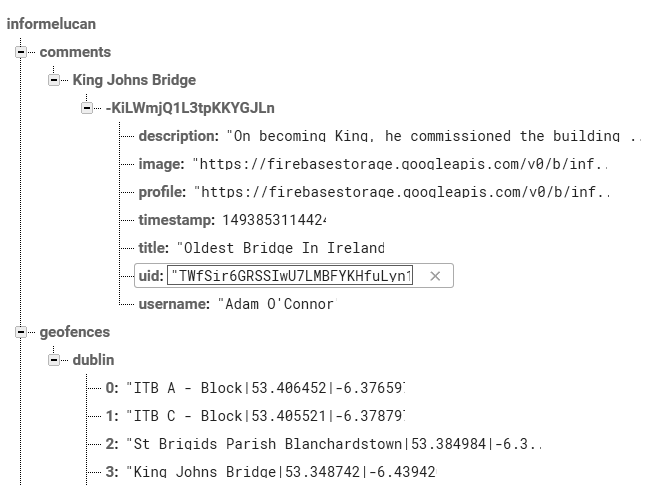
\includegraphics[width=300pt]{database1}\\
	\caption{Firebase Database} \label{Figure: Firebase Database}
	
	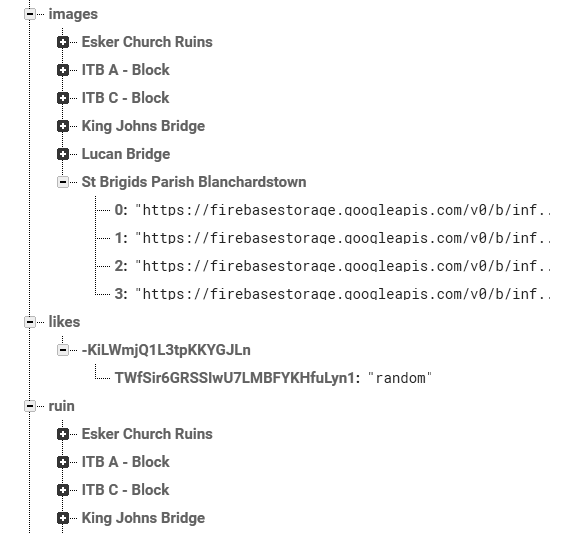
\includegraphics[width=300pt]{database2}\\
	\caption{Firebase Database} \label{Figure: Firebase Database}
\end{figure}

\newpage

\section{Summary of the Chapter}
Regarding the following chapter, the developer of the InforMe@Dublin Android application displayed and discussed some of the more important methods of the classes in the app. Most of the listings which are referenced by a unique identification number, regarding each of the methods and code snippets referenced above in the chapter the full code of the following application is supplied within the following thesis.
